\documentclass[10pt,twocolumn,letterpaper]{article}

\usepackage{cvpr}
\usepackage{times}
\usepackage{epsfig}
\usepackage{graphicx}
\usepackage{amsmath}
\usepackage{amssymb}
\usepackage{natbib}

% Include other packages here, before hyperref.

% If you comment hyperref and then uncomment it, you should delete
% egpaper.aux before re-running latex.  (Or just hit 'q' on the first latex
% run, let it finish, and you should be clear).
\usepackage[breaklinks=true,bookmarks=false]{hyperref}

\cvprfinalcopy % *** Uncomment this line for the final submission

\def\cvprPaperID{****} % *** Enter the CVPR Paper ID here
\def\httilde{\mbox{\tt\raisebox{-.5ex}{\symbol{126}}}}

% Pages are numbered in submission mode, and unnumbered in camera-ready
%\ifcvprfinal\pagestyle{empty}\fi
\setcounter{page}{4321}
\begin{document}

%%%%%%%%% TITLE
\title{Comparing Pixel Inputs and Structured Inputs in Reinforcement Learning with Self-Play}

\author{Brendon Go\\
Stanford University\\
{\tt\small go@cs.stanford.edu}
% For a paper whose authors are all at the same institution,
% omit the following lines up until the closing ``}''.
% Additional authors and addresses can be added with ``\and'',
% just like the second author.
% To save space, use either the email address or home page, not both
\and
Evan Liu\\
Stanford University\\
{\tt\small evanliu@cs.stanford.edu}
}

\maketitle
%\thispagestyle{empty}

\section{Introduction}

In the Reinforcement Learning (RL) paradigm, agents learn to perform complex
tasks through trial-and-error. The agents take certain actions and observe their
consequences -- learning to prefer actions that lead to positive consequences.
This paradigm has shown great promise in disparate applications, ranging from
dialogue generation \citep{dialogue2016}, to game playing \citep{mnih2015human},
to robotics \citep{robotics2016}.

Recent RL methods have achieved superhuman performance on Atari 2600 games
\citep{bellemare2013arcade}. These methods receive as input the raw pixels that
appear on the game screen, and output actions (e.g. moving left or right),
learning to find action sequences that maximize the game score. Traditional
wisdom posits that the task would be easier if the input were structured (e.g.
the positions of the character and enemies in the game) rather than pixels,
because with pixel inputs, the pixels must first be processed to extract this
structured information. However, surprisingly, on a version of the Atari 2600
games, where the inputs to the RL agent are the game memory (which include
information like the coordinates of the avatar), current RL methods perform
poorly, far worse than on the pixel version \citep{atariRAM}.

We investigate this phenomenon on games outside of Atari to determine
if the poor performance is an artifact of the structure of Atari games or if
there is a deeper reason. In particular, we focus on a favorite game from the
90s, Slime Volleyball, where the goal of the game is to hit a ball over a net
onto the opponent's side of the game. Players win points when the ball hits the
ground on the opponent's side of the net. We apply deep RL methods to
this game with two types of inputs: the pixels of the game screen, and the
variables used to generate the game, and compare the performance of these
algorithms on different types of inputs. Success on this project will hopefully
lend greater insight into why Atari on RAM states fails, possibly leading to
novel RL algorithms or insights about the pixel states.

\section{Problem Statement}
\subsection{Data}

We have modified an HTML5 implementation of Slime Volleyball, to use
as a browser-based simulation environment. We use Selenium to receive the
state from the browser and to send the agent's actions to the browser. To train
both a pixel-state and a structured-state model, we modify the simulator to be
able to generate both states.


\begin{figure}[h]
\center
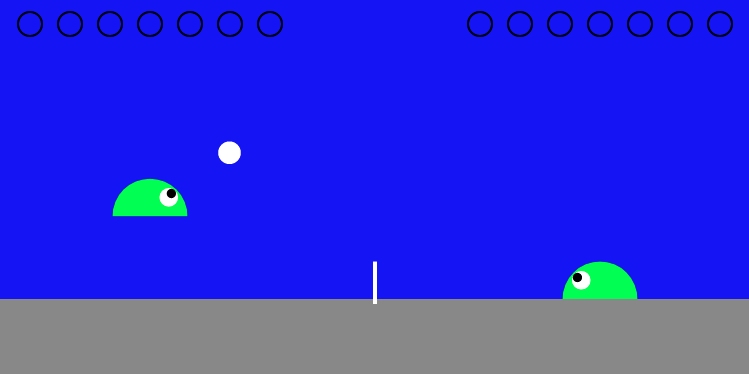
\includegraphics[width=\columnwidth]{SlimeVolleyBall}
\caption{
Player 1 Serving the ball over the net in Slime Volleyball
}\label{fig:slime}
\end{figure}

\subsection{Evaluation}

We define the result of a game to be the difference between our agents final score
and the opponents final score. The first agent to get 7 points wins the game.
Thus the results can range from $-7$ to $7$. Slime Volleyball has a one-player
version wherein the player fights against a hard-coded opponent. As a baseline
we calculate the average result of a human player against the hard-coded opponent. \\

\noindent We evaluate our agent by taking its average result over 100
games. We will be able to compare our two models by comparing their respective
results.

\noindent We think it will also be worthwhile to pit the two models against each
other in the two player variant of slime volleyball and seeing if the average
result over 100 games leans one way or the other.

\section{Technical Approach}

\subsection{Method} We will implement Deep Q-Networks as our policies. Briefly,
Q-Networks associate with each state $s$ and each action $a$ and value $Q(s, a)$
estimating the reward that the network will receive for playing action $a$ in
state $s$. A policy can be recovered from this by playing the action $a$ with
the highest $Q$ value at each state $s$. These Q-Networks will learn via self-
play.

\section{Intermediate/Preliminary Results}

Here are results



{\small
\bibliographystyle{unsrtnat}
\bibliography{egbib}
}

\end{document}
